% Dieser Text ist urheberrechtlich gesch�tzt
% Er stellt einen Auszug eines von mir erstellten Referates dar
% und darf nicht gewerblich genutzt werden
% die private bzw. Studiums bezogen Nutzung ist frei
% Januar 2006
% Autor: Sascha Frank 
% Universit�t Freiburg 
% www.informatik.uni-freiburg.de/~frank/
% www.namsu.de/


\documentclass[xcolor=dvipsnames]{beamer}
\usetheme{CambridgeUS}
\usepackage[ngerman]{babel}
\usecolortheme{seagull}  
\usefonttheme{default}
%\usepackage[center]{caption}

\useoutertheme{infolines}
\useinnertheme{rectangles}

\usepackage{tikz}
\usetikzlibrary{positioning}
%\usepackage{mathptmx}
\usepackage{cancel}
\usepackage{appendixnumberbeamer}
\usepackage{changepage}
\usepackage{subfig}
%\usepackage{subcaption}

\title{The title}
\institute[]{~}
\date{\today}

\def\thisframelogos{}

\newcommand{\framelogo}[1]{\def\thisframelogos{#1}}

%\addtobeamertemplate{frametitle}{}{%
%	\begin{tikzpicture}[remember picture,overlay]
%	\node[anchor=north east,yshift=-8pt] at (current page.north east) {%
%		\foreach \img in \thisframelogos {%
%			\hspace{.5ex}%
%			\includegraphics[height=0.8cm]{\img}%
%		}%
%	};
%	\end{tikzpicture}}

%\setbeamercolor{alerted text}{fg=orange}
%\setbeamercolor{background canvas}{bg=white} %Hintergrund
%\setbeamercolor{block body alerted}{bg=normal text.bg!90!black} %BL�cke 
%%(block, exampleblock, alterblock)
%\setbeamercolor{block body}{bg=normal text.bg!90!black}
%\setbeamercolor{block body example}{bg=normal text.bg!90!black}
%\setbeamercolor{block title alerted}{use={normal text,alerted text},fg=alerted 
%text.fg!75!normal text.fg,bg=normal text.bg!75!black}
%\setbeamercolor{block title}{bg=blue} %Block hintergrund 1 
%\setbeamercolor{block title example}{use={normal text,example text},fg=example 
%text.fg!75!normal text.fg,bg=normal text.bg!75!black} %blok hintergrund 2
%\setbeamercolor{fine separation line}{}
%\setbeamercolor{frametitle}{fg=black} %frame titel
%\setbeamercolor{item projected}{fg=black}
%\setbeamercolor{normal text}{bg=black,fg=yellow}
%\setbeamercolor{palette sidebar primary}{use=normal text,fg=normal text.fg}
%\setbeamercolor{palette sidebar quaternary}{use=structure,fg=structure.fg}
%\setbeamercolor{palette sidebar secondary}{use=structure,fg=structure.fg}
%\setbeamercolor{palette sidebar tertiary}{use=normal text,fg=normal text.fg}
%\setbeamercolor{section in sidebar}{fg=brown}
%\setbeamercolor{section in sidebar shaded}{fg=grey}
%\setbeamercolor{separation line}{}
%\setbeamercolor{sidebar}{bg=blue}
%\setbeamercolor{sidebar}{parent=palette primary}
\definecolor{darkred}{rgb}{0.8,0,0}
\setbeamercolor{structure}{bg=white, fg=darkred}
%\setbeamercolor{subsection in sidebar}{fg=brown}
%\setbeamercolor{subsection in sidebar shaded}{fg=grey}
%\setbeamercolor{title}{fg=brown}
%\setbeamercolor{titlelike}{fg=brown}

\setbeamertemplate{itemize items}[default]


 %\renewcommand{\figurename}{}

\defbeamertemplate*{sidebar right}{CambridgeUS}
{
	\vskip2pt%
	\llap{\insertlogo\hskip0.2cm}%
	\vfill
	\llap{\usebeamertemplate***{navigation symbols}\hskip0.2cm}%
	\vskip2pt%
}
%\setbeamertemplate{caption}{\raggedright\insertcaption\par}
\captionsetup[figure]{labelformat=empty}
\usepackage{lmodern}               
\usepackage{mathptmx}
%\usepackage{tpslifonts}
%\usepackage[perpage]{footmisc}
\begin{document}


\title[~]{Giant spike count variability in two-dimensional Neuron models} 
\author{Richard Kullmann} 
\date{31 March 2020}
%\logo{
\includegraphics[scale=0.14]{husiegel}}
%\framelogo{husiegel}


\begin{frame}
\titlepage
\end{frame}
\section{Introduction}
\subsection{Neurophysics}
\begin{frame}{Neurons and Bursting}
\begin{itemize}
	\item 100 billion neurons in human brain%\cite{eqnum}
	\item neurons transmit information via spiking activity
	\item spike = abrupt change of membrane voltage (action potential) that propagates through axon 
\end{itemize}
\begin{figure}[H]
	\captionsetup[subfigure]{labelformat=empty}
	\subfloat[]{
\includegraphics[scale=0.27]{intburyaxis.png}} 
	\subfloat[]{	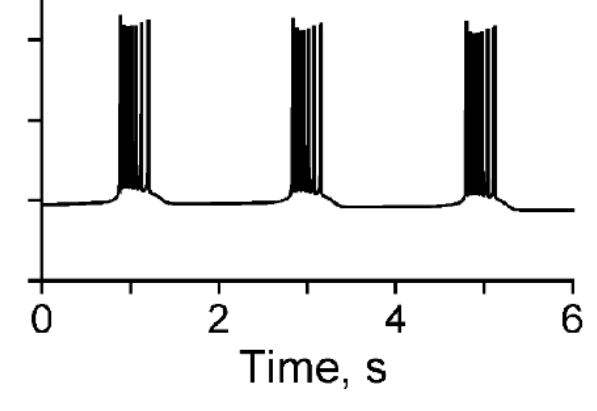
\includegraphics[scale=0.3]{intburnox.png}}
	\vspace{-0.5cm}
	\caption{intrinsic bursting in a pacemaker neuron model (Rybak, 2004)}
	\label{intbur} 
\end{figure}
%	\begin{figure}[H]
%		\subfigure[]{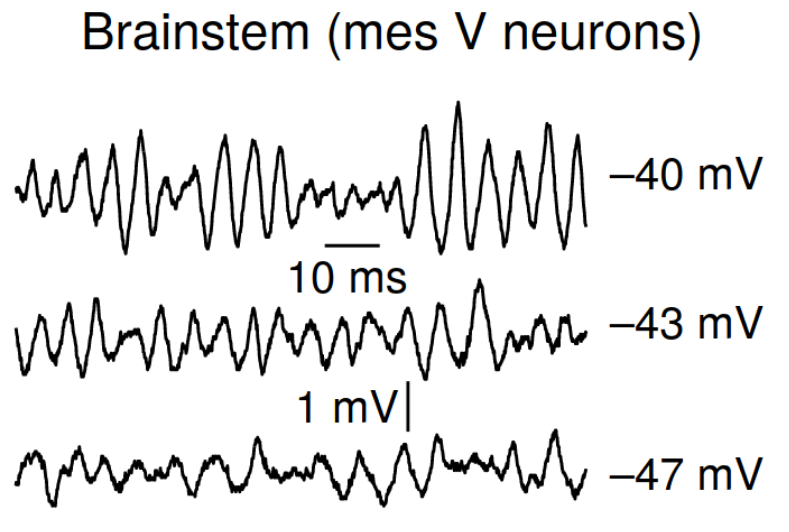
\includegraphics[scale=0.15]{subthrizi.png}
%		\label{subthr}} 
%	\vspace{0.5cm}
%		\subfigure[]{	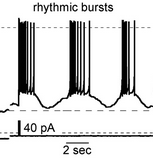
\includegraphics[scale=0.6]{26.png}
%		\label{fig26}}
%		\caption{neuronal measurements of sub-threshold oscillations\cite{subthrizi} (left) and bursting\cite{burstpic}}
%		\label{subfig} 
%	\end{figure}	
%\footnotetext[1]{E. M. Izhikevich et al, "Bursts as a unit of neural information:selective communication viaresonance,"\textit{Trends in Neurosciences 26}, 2003.}
%\footnotetext[2]{Jason I. Kass and Isabelle M. Mintz, "Silent plateau potentials, rhythmic bursts, and pacemaker firing: Three patterns of activity that coexist in quadristable subthalamic 		neurons,"\textit{PNAS Vol. 103}, 2006.}
\end{frame}
\subsection{Topic}
\begin{frame}{Goals of this project}
\begin{itemize}
	\item Overall goal: simulate bursting in simple neuron models and investigate spike count statistics
	\item in comparable systems (Brownian Particles, Lindner/Sokolov, 2016) critical points where firing pattern changes drastically\\ $\rightarrow$can we find these here as well?
	\item simulate neurons under influence of periodic stimulus to explore signal transmission
\end{itemize}
\end{frame}
%\begin{frame}{Bursting}
%\begin{itemize}
%\begin{columns}[t]
%	\column{.45\textwidth}
%	\item intrinsic bursting: once the system is brought into a bursting state, it can sustain it without needing further input
%	\centering
%%	\vspace{-0.5cm}
%	\begin{figure}
%		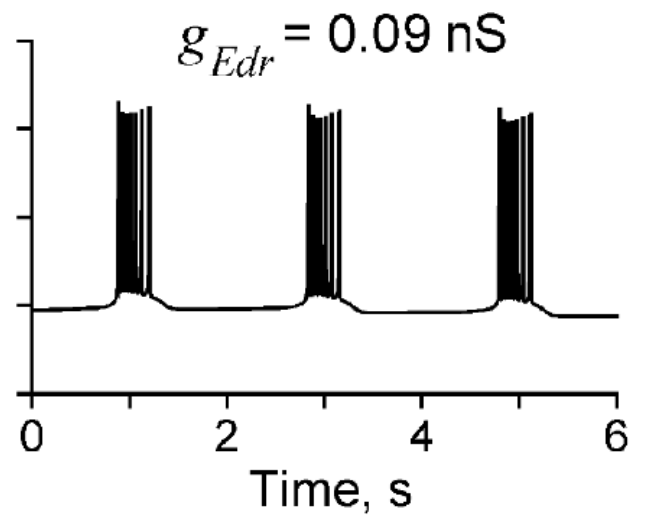
\includegraphics[scale=0.15]{intbur.png}
%		\caption{intrinsic bursting in a pacemaker neuron model\cite{intburst}}
%		\label{intbur}
%	\end{figure}
%	\column{.45\textwidth}
%	\item input-driven bursting: neuron does only exhibit bursting under certain external stimuli
%	\centering
%%	\vspace{-1cm}
%	\begin{figure}
%		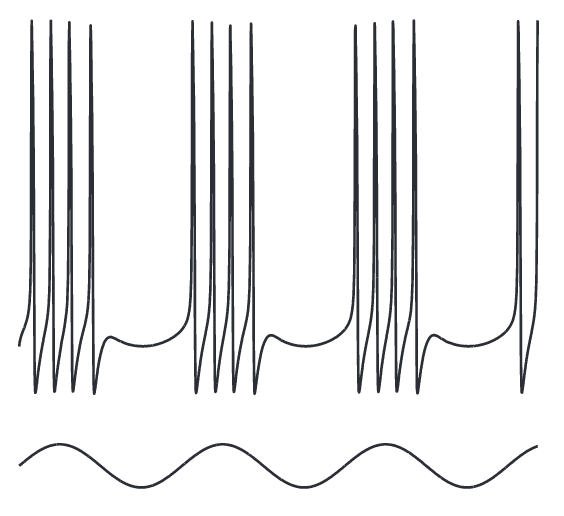
\includegraphics[scale=0.2]{forcedbur.png}
%		\caption{illustration of forced bursting via a periodic signal \cite{izi}}
%		\label{forcedbur}
%	\end{figure}
%\end{columns}
%\end{itemize}
%\end{frame}
%\begin{frame}{Bistable neurons}
%\begin{itemize}
%%\item station"are L"osung $\left(\text{mit} -U'(v)=f(v)/g^2(v)\right)$:
%%\begin{equation}\nonumber
%%P_0(v)=\frac{\text{e}^{-U(v)/Q}/g^2(v)}{|| \cdot ||}
%%\end{equation}
%\item two regimes of neural activity in single neuron
%\item of special interest: coexistence of resting and spiking state
%\item short pulses of current cause change of state 
%$\rightarrow$ stochastic bursting is induced when noise makes neuron switch between both configurations
%\begin{figure}
%	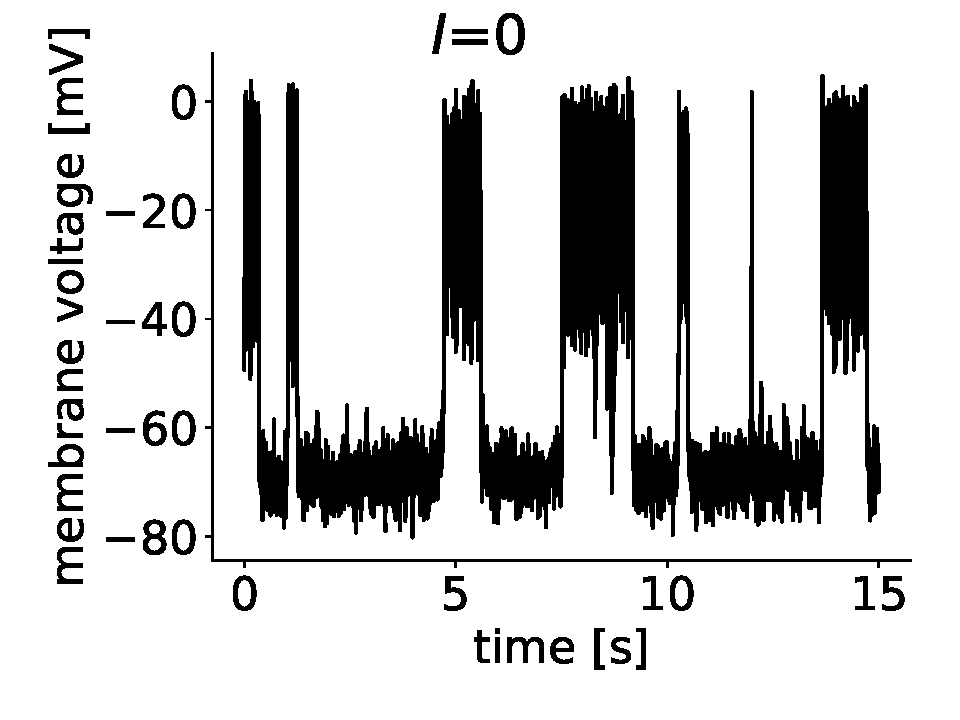
\includegraphics[scale=0.4]{realstatevar1352.pdf}
%\end{figure}
%\end{itemize}
%\end{frame}
%\begin{frame}{Noise sources}
%\begin{itemize}
%	\item \textit{channel noise}: finite-size noise caused by probabilistic gating of voltage-dependent ion channels
%	\item unreliable synapses, due to variability in amplitudes of synaptic potentials, transmission failure and spontaneous release of neurotransmitters
%	\item largest source of stochasticity: quasi-random input from other neurons
%\end{itemize}
%\end{frame}
\section{Neuron model}
\subsection{$I_{Na,p}+I_K$ model}
%\begin{frame}{Persistent sodium plus potassium model}
%\begin{itemize}
%	\item simplest model for (stochastic) bursting: 2-D neuron model+noise
%	\item $I_{Na,p}+I_K$ model:
%	\begin{align*}
%	\hspace*{-2cm}
%	C\dot{V} &= I - g_L(V-E_L) - g_{Na}m_{\infty}(V)(V-E_{Na}) - g_Kn(V-E_K)+\sqrt{2D}\xi(t)\\\label{neq}
%	\dot{n} &= (n_{\infty}(V)-n)/\tau(V)
%	\end{align*}
%	$C$...capacitance\\
%	$I$...bias current\\
% $g_i$...conductances\\
% $E_i$...ionic equilibrium potentials\\
%$n_\infty$,$m_\infty$...sigmoid-shaped activation functions\\
%$n$...gating variable of potassium channels\\
%$D$...noise intensity\\
%$\tau$...voltage-sensitive time constant
%	
%\end{itemize}
%\end{frame}
\begin{frame}{Persistent sodium plus potassium $I_{Na,p}+I_K$ model}
\begin{itemize}
	\item simplest model for (stochastic) bursting: 2-d neuron model+noise
	\item electric activity in neurons relies on ionic currents through membranes
	\item $I_{Na,p}+I_K$ model:
	\begin{align*}
	\hspace*{-2cm}
	C\dot{V} &= I_{bias} - I_L - I_{Na} - n\cdot I_K+\sqrt{2D}\xi(t)\\\label{neq}
	\dot{n} &= (n_{\infty}(V)-n)/\tau
	\end{align*}
	$V$...membrane voltage\\
	$n$...gating variable of potassium channels\\
	$C$...capacitance\\
	$I_L$...leak current\\
	$n_\infty$...sigmoid-shaped activation function\\
	$D$...noise intensity
	
\end{itemize}
\end{frame}
%\begin{frame}{Nullclines}
%\begin{itemize}
%	\item curves where one state variable remains constant
%	\begin{figure}[H]
%		\centering
%		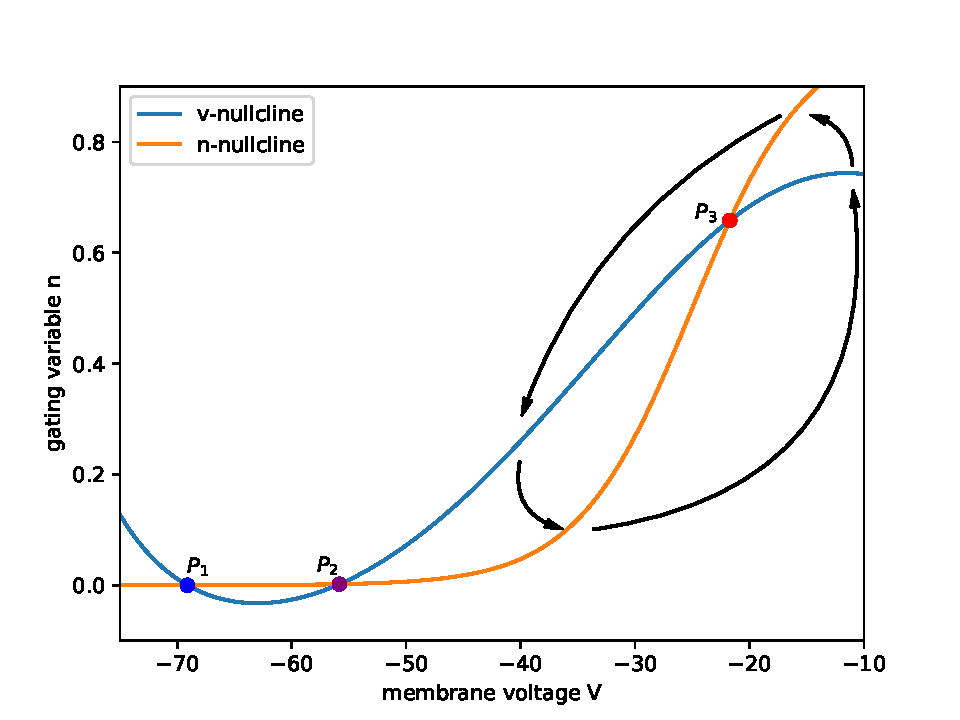
\includegraphics[scale=0.5]{inapikrealncwnp.pdf}\caption{Nullclines of the $I_{Na,p}+I_K$-model. The arrows indicate the direction of motion in the different regions.}
%		\label{realnc}
%	\end{figure}
%\end{itemize}
%\end{frame}
%\begin{frame}{System without noise}
%\begin{figure}[H]
%	\captionsetup[subfigure]{labelformat=empty}
%	\vspace{-0.5cm}
%	\subfloat[]{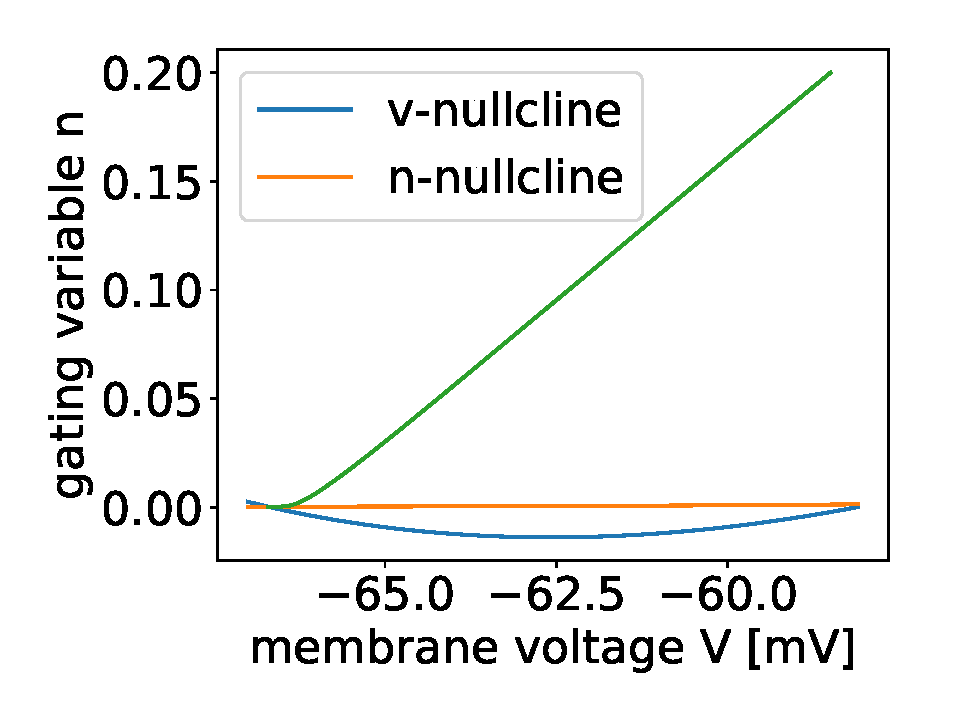
\includegraphics[scale=0.3]{inapreali20nbwnfont.pdf}} 
%	\subfloat[]{	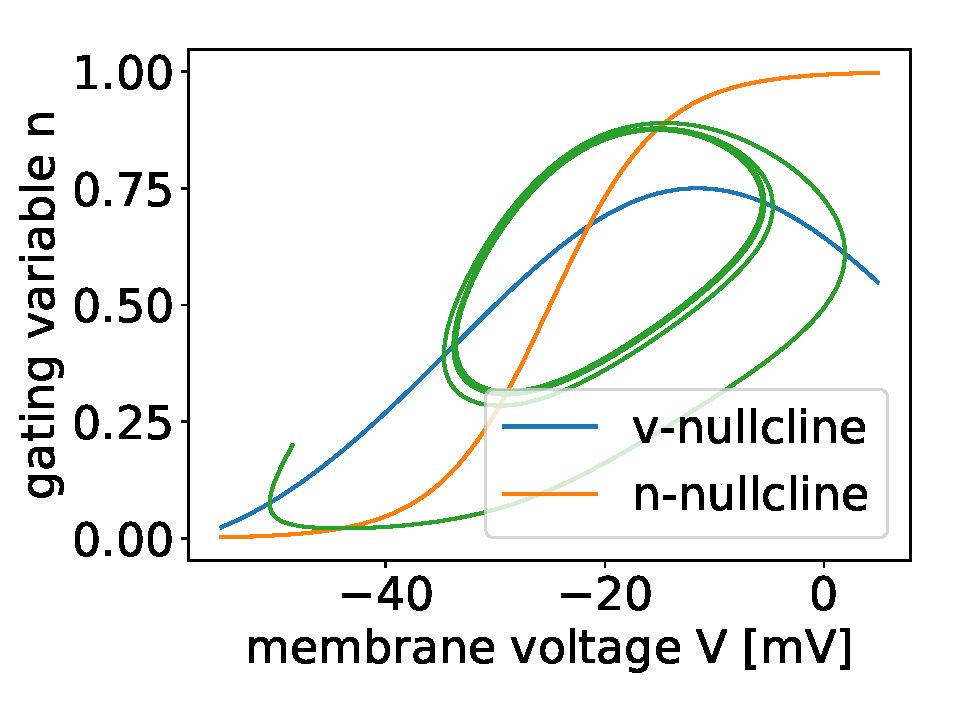
\includegraphics[scale=0.3]{inapreali20wnfont.pdf}}\\
%	\vspace{-1cm}
%		\subfloat[]{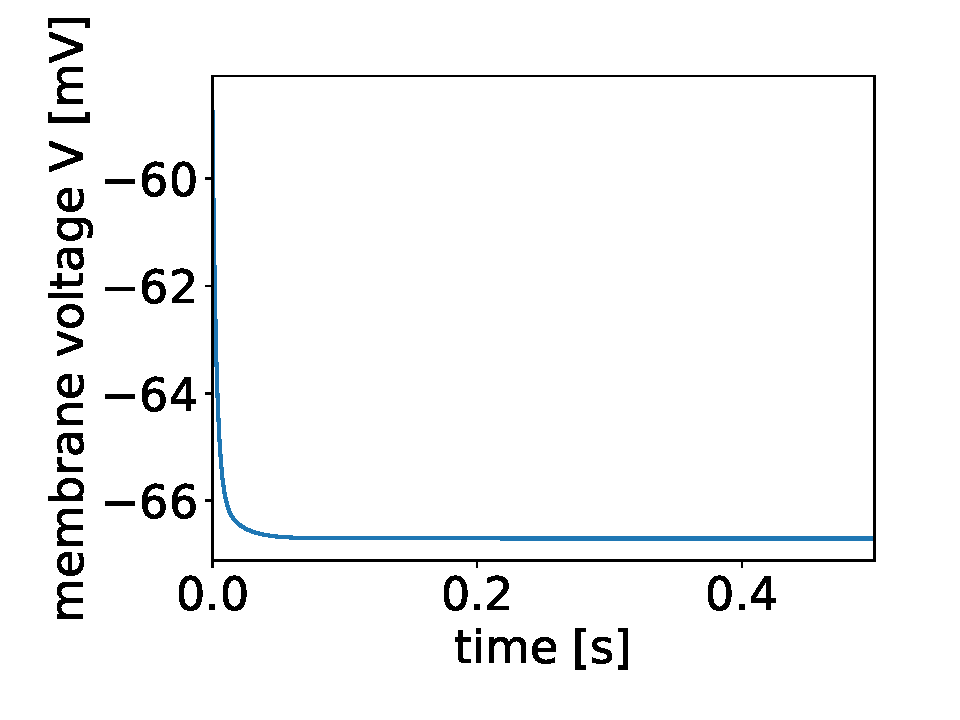
\includegraphics[scale=0.3]{inapreali20nbvfont.pdf}} 
%	\subfloat[]{	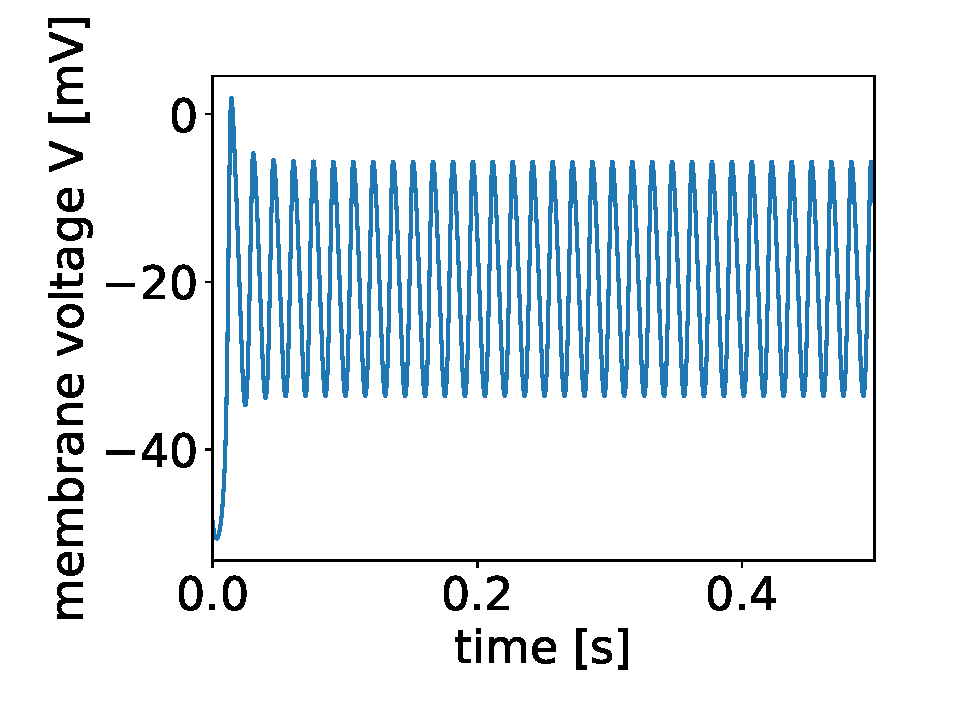
\includegraphics[scale=0.3]{inapreali20vfont.pdf}}
%	\label{subfig} 
%\end{figure}
%\end{frame}
\begin{frame}{Membrane voltage}
\begin{itemize}
	\item system is bistable: resting and spiking states coexist
	\item noise induces transitions between states
	\item higher bias current favors spiking state\\ $\rightarrow$ neuron bursts longer and more frequently:
\end{itemize}
\begin{tikzpicture}
%		\captionsetup[subfigure]{labelformat=empty}
\node (1) {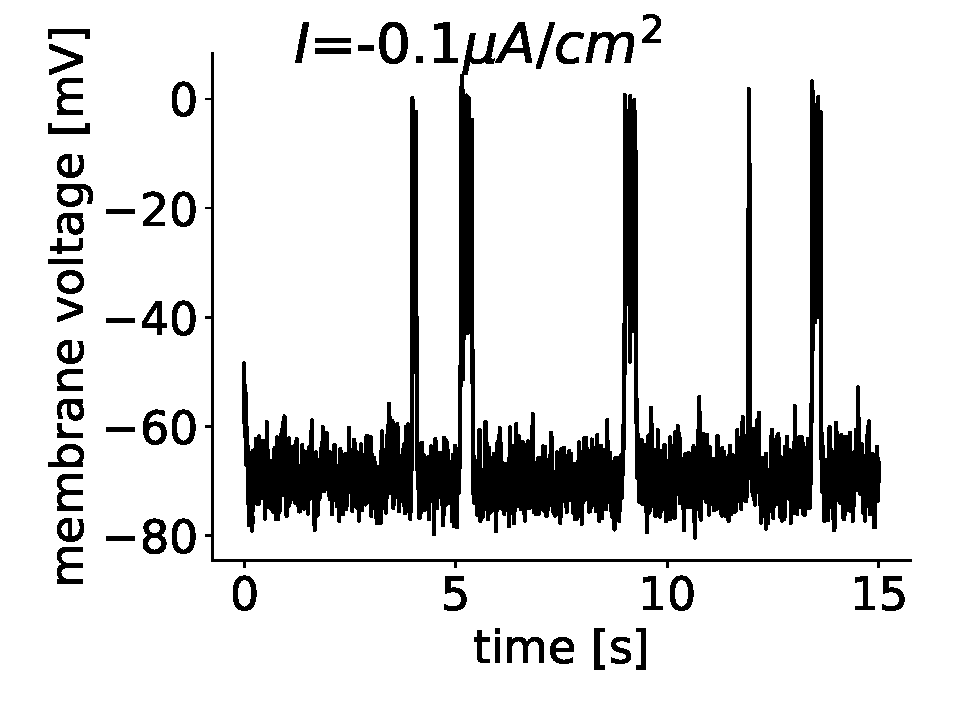
\includegraphics[scale=0.3]{realstatevar1252.pdf}};	
\node (3) [right=of 1] {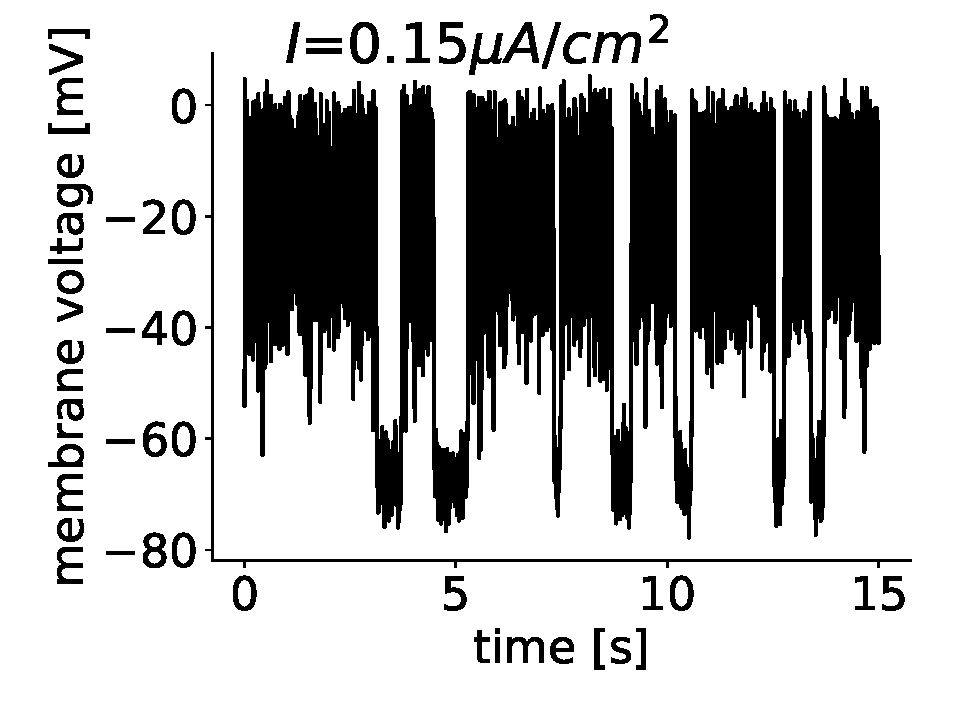
\includegraphics[scale=0.3]{realstatevar152.pdf}};
\draw [ultra thick,magenta,->] (1) to (3);
	%\\	\subfloat[]{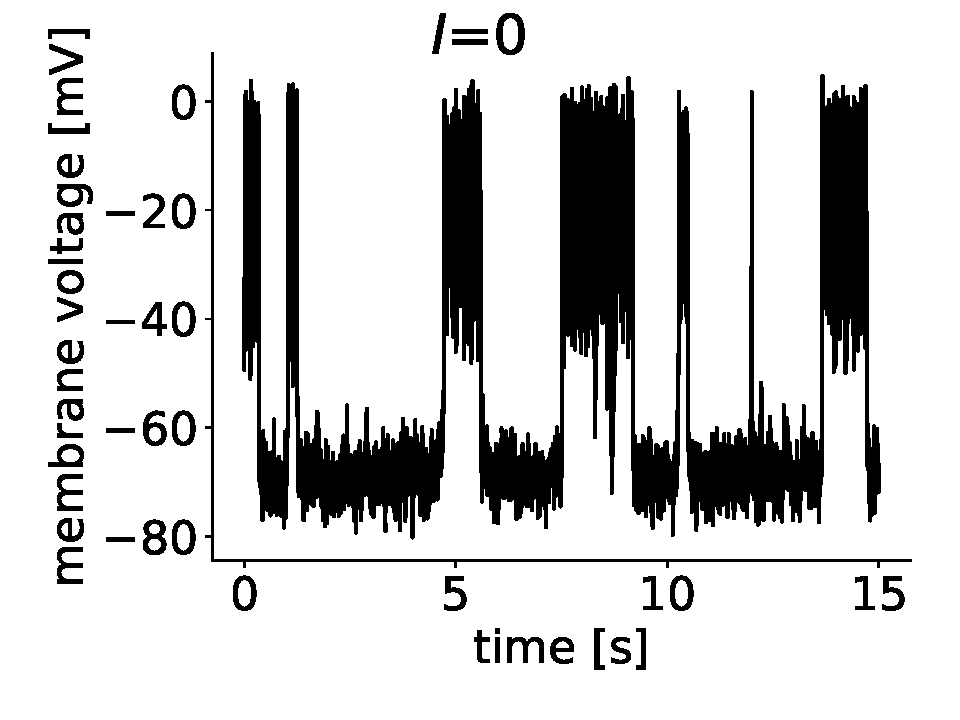
\includegraphics[scale=0.25]{realstatevar1352.pdf}} 
	%\subfloat[]{	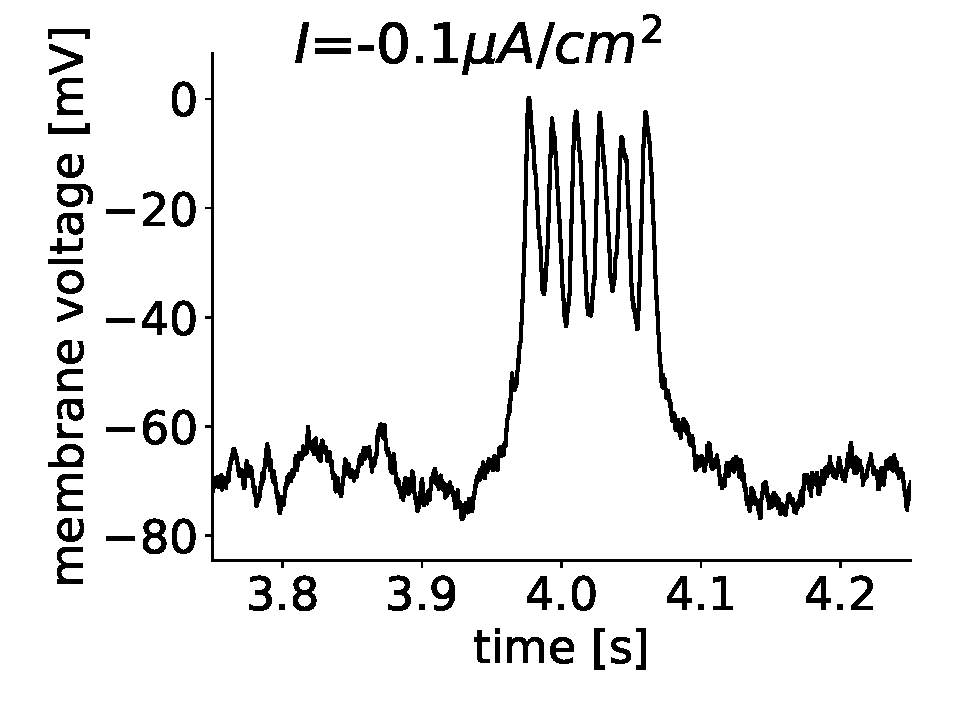
\includegraphics[scale=0.25]{realstatevar125vsh2.pdf}}
\end{tikzpicture}
\end{frame}
\begin{frame}{Quantities of interest}
\begin{itemize}
\item System without signal
\begin{itemize}
	\item spike count $N(t)$: number of spikes after time $t$
	\item spiking variability quantified by Fano factor: $
	F(t)=\frac{\left\langle \Delta N^2(t) \right\rangle}{\left\langle N(t)\right\rangle}
	$
\end{itemize}
\end{itemize}
\begin{itemize}
	\item System with periodic signal 
\begin{itemize}
	\item power spectrum $S(f)$ measures frequency of components in membrane voltage
\item signal-to-noise ratio (SNR) compares power of signal to background noise
\item weak+slow signal= $SNR\propto1/F$\\
$\rightarrow$ changes in Fano factor $F$ have opposite effect on SNR
\end{itemize}
\end{itemize}
\end{frame}
\section{Measurements}
\begin{frame}{Count statistics}

	\begin{figure}[H]
		\centering
		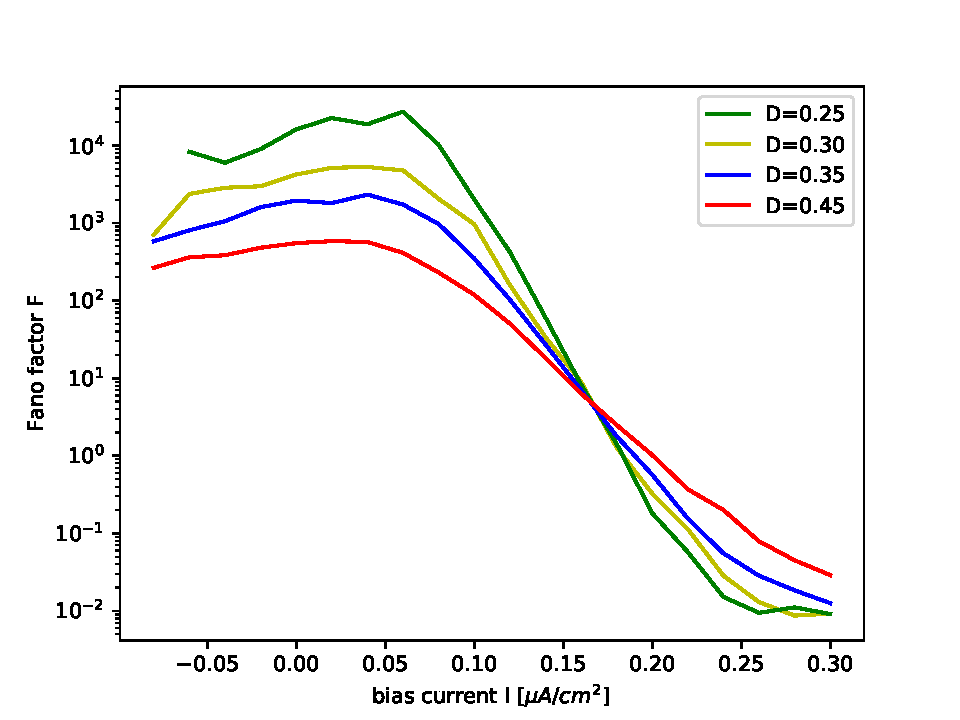
\includegraphics[scale=0.5]{fneur3shrealfast19jjem2strealfast13aem2n4realfast11jjem2sh.pdf}
		\label{fano}
		\caption{Fano factor at different noise intensities $D$. The intersection point forms the border between giant (left) and small (right) Fano factor $F$ in the $D\rightarrow0$ limit.}
	\end{figure}

\end{frame}
%�
\begin{frame}{Power spectrum for system with signal}
	\begin{figure}[H]
	\centering
	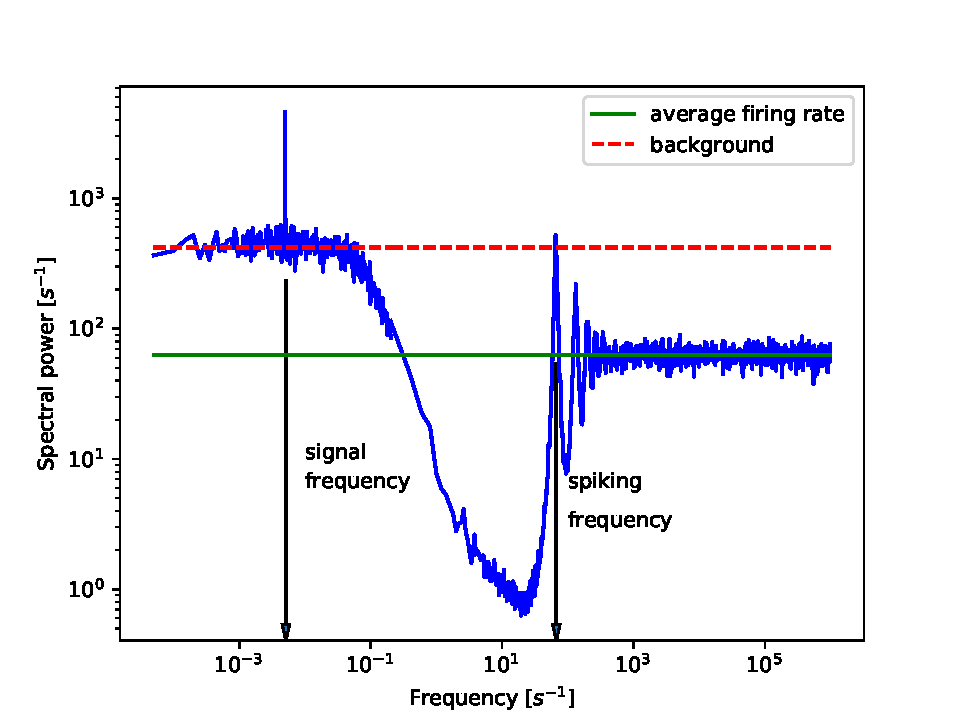
\includegraphics[scale=0.5]{specimprs.pdf}
	\caption{Power spectrum of the membrane voltage. A sharp spike can be seen at the signal frequency ($5\cdot10^{-3}$Hz) and a second maximum at the spiking frequency($10^2$Hz)}
	\label{specglue}
\end{figure}
\end{frame}
\begin{frame}{Signal-to-noise ratio SNR}
	\begin{figure}[H]
	\centering
	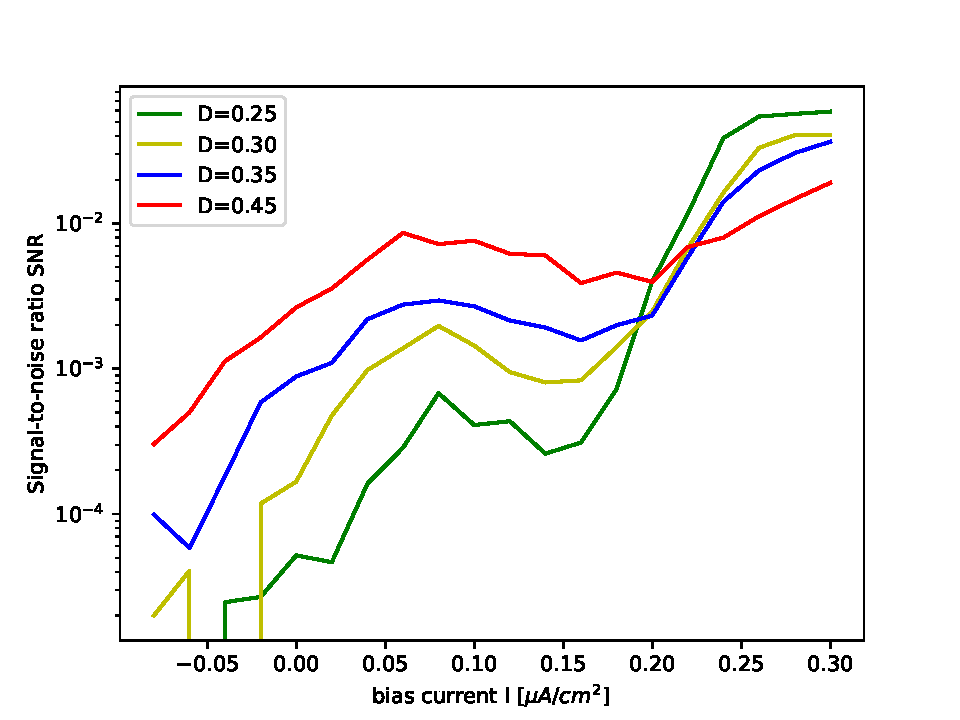
\includegraphics[scale=0.5]{snrealonly.pdf}
	\caption{SNR at different noise intensities. As expected, a sharp increase is observed where Fano factor $F$ becomes minimal.}
	\label{snronly}
\end{figure}
\end{frame}
\section{Conclusion}
\begin{frame}{Conclusion}
\begin{itemize}
	\item two-dimensional bistable neuron model turned into burster by adding noise
	\item critical current observed where Fano factor $F$ drops strongly
	\item SNR grows by multiple orders of magnitude near critical current\\
	$\rightarrow$ bistable neurons in the critical regime can greatly enhance signal transmission via slight adjustment of currents
\end{itemize}
\end{frame}
%\begin{frame}
%\bibliography{quellenimprs}
%\bibliographystyle{ieeetr}
%\end{frame}
\end{document}

